	The state-transition modelling approach is our proposal to better address the routing requirements involving design-code equivalence and adaptability criteria (see Section \ref{sec:literature:flowParadigm}). This model, widely used for the specification of reactive systems \cite{tech:androutsopoulos08}, is inspired by the \gls{efsm} \cite{book:alagar11}.

	An example of the state-transition model, represented in Figure \ref{fig:design:stateTransition}, describes the questionnaire presented in Figure \ref{fig:background:survey}. It contains various types of states, represented by ellipses, that are linked through transitions to form state models (e.g. the Outer and Inner rectangles). 

	Each state model contains variables that reference questions defined in a section (e.g. INF1, Q1, Q2, Q3, Q4, Q5, INF2 and END for the Outer section or Q6a for the Inner). The scope of these is local to a state model and therefore their references do not exist outside. In order to reference variables through any state model, this paradigm defines global place holders, known as fields, that permit sharing data across different parts of a questionnaire (e.g. HAD\_CAR describing an integer number of cars that the respondent had).

	The states are addressed to perform single operations and these may be categorised as follows:

	\begin{itemize}
		\item \emph{Simple} states are used to present the questions to the respondent and to store responses in variables (e.g. every state prefixed with 's').
		\item \emph{Composite} states refer to a defined state model (e.g. c0 and c1 for Outer and Inner state models respectively) and are useful for reducing coupling among questions in a survey.
		\item Pseudo states are normally used to take routing path decisions through the evaluation of boolean expressions. Specifically, there are \emph{if} and \emph{for} states to decide the conditions under which questions are asked and \emph{check} states to validate inconsistent responses. Additionally, the \emph{computation} state unlike its counterparts is utilised to update place holder variables through \emph{arithmetic} expressions.
	\end{itemize}

	The transitions connect a state source with a state target to create a questionnaire's flow (e.g. arrows connect ellipses). If a transition does not define a boolean expression, it is assumed true whenever the state source of the transition is reached. In contrast, if a boolean expression is defined, this means that the expression has to be evaluated in order to determine its truth (e.g. Q1 '01' IS\_SEL Q1 '02' IS\_SEL OR Q1 '03' IS\_SEL OR). Here we propose the use of postfix notation mode as the expression formalism for all the expressions used in the design of a questionnaire.

	The state models have an initial state that determines what state is executed first (e.g. s0 and s8 for Outer and Inner respectively) as well as one or more ending states (e.g. 'sink0', 'sink1' or 'sink2'). Similarly, the state-transition model requires a state model that marks the beginning, i.e. an entry point for the model to capture a questionnaire's flow (e.g. 'c0' and 'sink0' states).

	%Our model reacts to a two types of events: \emph{external}, which occurs whenever a respondent requests moving forward or backward through a questionnaire; and \emph{internal} that is triggered every time a variable is updated. This updating forces an automatic re-evaluation of every expression that contains a reference to that variable. This is possible as X adopts the Observer pattern design implementation. %(see Appendix \ref{sec:design:observerPattern}).

	Accordingly, we formalise the state-transition model that is applied to questionnaire routing as follows:

	\begin{equation}\label{design:eqn:stateTransition}
		M = \langle Q,V,T,I,E \rangle
	\end{equation}
	where,
	\begin{enumerate}
		\item $Q(\neq \emptyset)$ is a finite set of states.
		\item $V$ is the set of state variables. Every variable $x \in V$ may be accessed at every state $q \in Q$.
		\item $T$ is a finite set of transitions. A transition $t \in T$ is represented as $q \xrightarrow{[c]} 
		q'$, where $\{q,q'\} \in Q$ and c is a boolean expression involving variables of $V$ defined in pre-state \emph{q}. The absence of $c$ is interpreted to true.
		\item $I\subset Q$ is the set of initial states. Every composite state has an initial state and consequently there is a set of initial states if the model contains composite states.
		\item $E\subset Q$ is the set of end states. These states may be \emph{sink} addressed to finish a state model or \emph{terminate} to interrupt and finish the execution of a state-transition model.
	\end{enumerate}

	\begin{figure}[H]
	\centering
	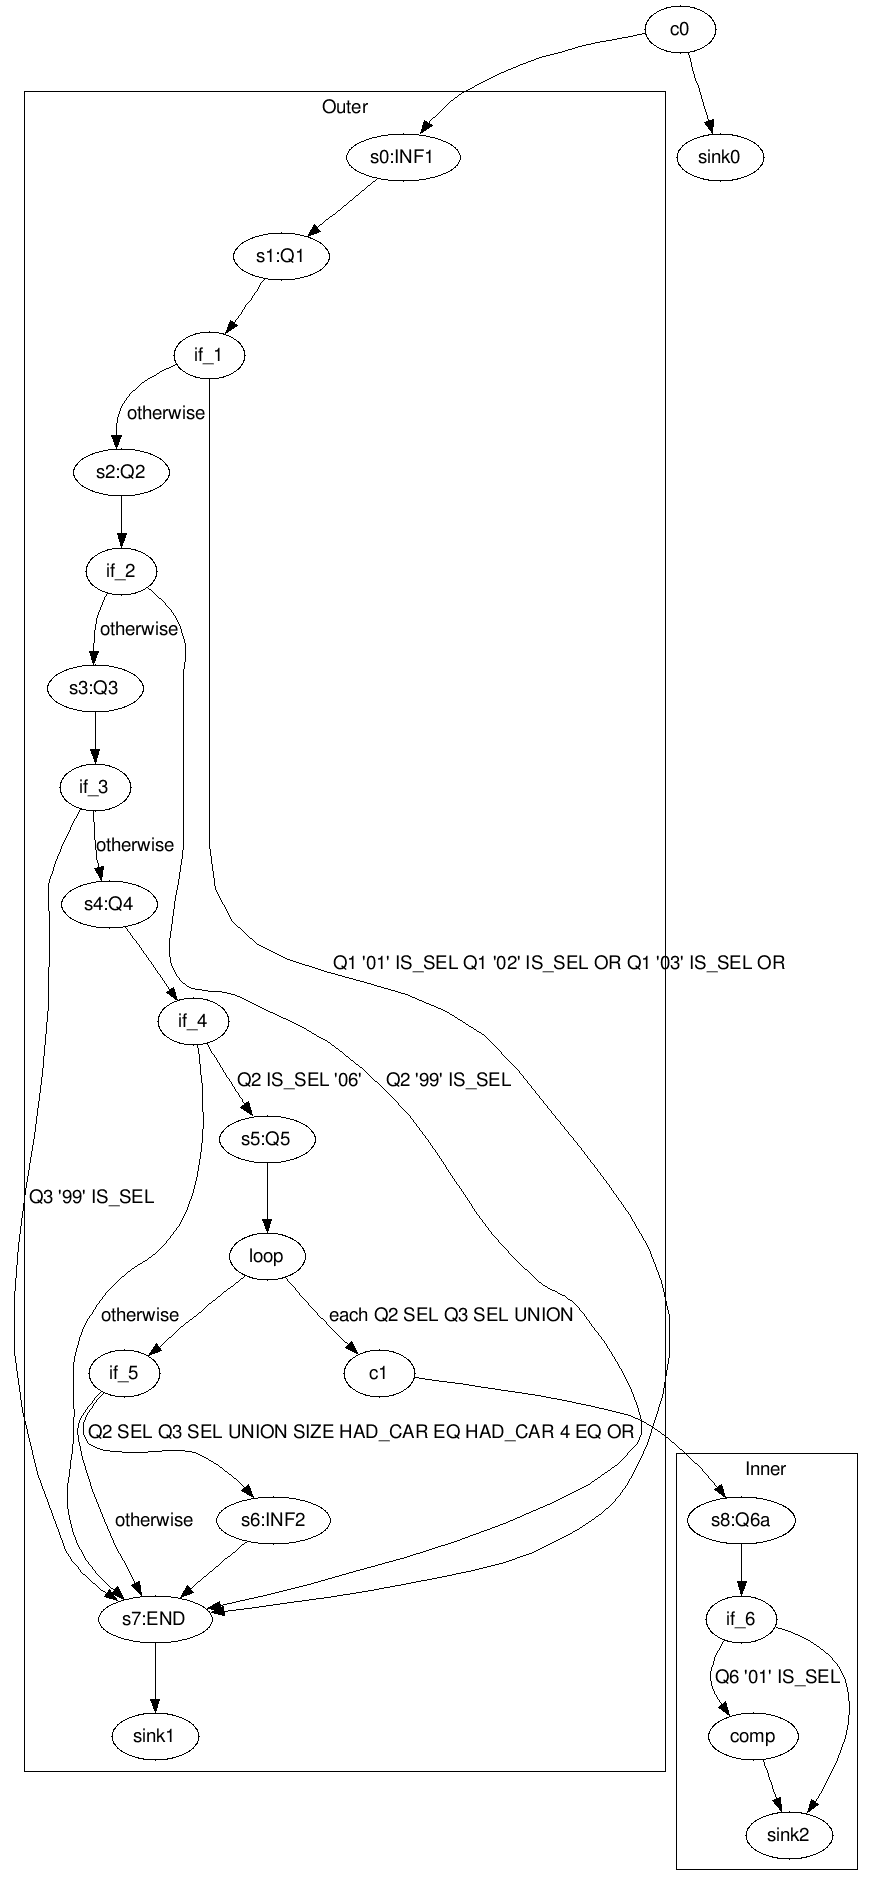
\includegraphics[max size={\textwidth}{\textheight}]{design/img/stateTransition.png}
	\caption{State-Transition for the paper questionnaire in Figure \ref{fig:background:survey}}
	\label{fig:design:stateTransition}
	\end{figure}

	%Our proposal for modelling questionnaire's routing does not explicitly defines skip constructs but it does not mean that the task of negating expressions has to be performed since this model does not rely on sequence lines which allows moving from one state to another by using transitions. Also as there is no possibility to define parent-child hierarchies among states, this potentially reduces the coupling of the routing constructs.

	



